%% Useful packages
\usepackage{amsmath}
\usepackage{graphicx}
\usepackage[colorinlistoftodos]{todonotes}
\usepackage[colorlinks=true, allcolors=blue]{hyperref}

\title{Stat 159 Final Project-School Performance Comparison}
\author{Atul Lanka,Timothy Park,Rushil Seth, Yuyu Zhang}

\begin{document}
\maketitle

\begin{abstract}
This project consists of performing a virtual consulting analysis from College ScoreCard data. Specifically, our team members analyzed and interpreted the data by EDA analysis, regression model building and interactive shiny app to help a group of art institution administrators to compare themselves with similar schools in California, in terms of diversity of graduation rates.
\end{abstract}

\section{Introduction}
\paragraph{Data Analysis has been extensively used in different areas to explore, understand and predict our daily life. The motivation behind this project is to provide insights for higher education officials/policymakers to better assess how well institutions are providing access to diverse group of students.  Our team decides to help a group of 4-year art institution administrators to compare themselves to similar schools in California, in terms of diversity and graduation rates.}

\paragraph{The overall workflow can be summarized as followed: data cleaning (target schools that are 4-year art institutions located in California)--> EDA Analysis( provide overall pictures of schools enrollment and graduation statistics)-->Model Building()--> Shiny App (interactive tool for user to visualize data with selected school and other criteria)-->Presentation slides( share results with public). Each section of the workflow will be explored and explained in details. }


\section{Data Cleaning}

\paragraph{The raw data used in this project comes from College ScoreCard, downloaded \href{https://ed-public-download.apps.cloud.gov/downloads/Most-Recent-Cohorts-All-Data-Elements.csv}{here}, developed by the U.S Department of Education. To select targeted school, we choose specifically four-year art schools in CA (these are indicated by the abbreviation "CCBASIC==30" and "STABBR=="CA" respectively in the raw data). We also extracted schools' location, zip code, website etc in similar way.}

\paragraph{ There are several indicators for diversity, which we identified as gender, average family income, average age and ethnicity. For the dependent variables, we choose enrollment and graduation rates. We further divide enrollment based on ethnicity (enroll-white is percentage of enrolled people that are white etc), gender(enroll-men etc), graduation based on ethnicity(grad-rate-asian etc). Note that the raw data doesn't provide graduation based on gender. We also catalog schools based on their region (1 indicates North Cal, 2 Central Cal and 3 for South Cal).} 
 \paragraph{Based on the criteria, 31 schools in total are selected and the finalized data is presented in "client-dat.csv".}


\section{EDA Analysis}
 \paragraph{ As the first step of data analysis, EDA tries to provide a general picture of average school performance. A picture is worth a thousand words, so let's take a look at what information the data discloses.}
  
 \begin{figure}
\centering
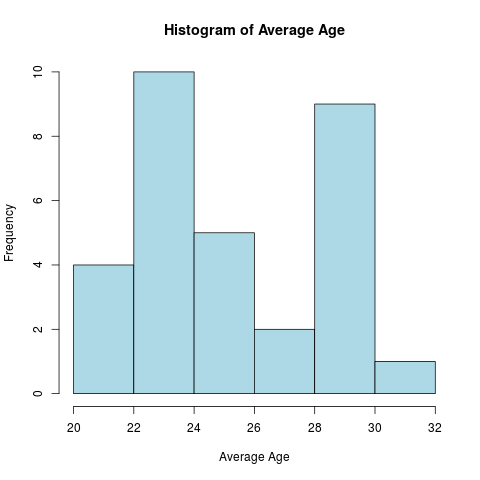
\includegraphics[width=0.5\textwidth]{histogram-age.png}
\caption{Average Age of Enrolled Students}
\end{figure}  
 
 \paragraph{Figure 1 shows enrollment rate vs average age. We can see two peaks at 22-24 and 28-30. It's expected that most people will choose to pursue a professional art degree after college, potentially as a way to change their career path (majority of universities/college don't have specialized art/design program). There's also a scenario where after working for several years, people decides to go back to school either for career switch or further their knowledge and skills.} 

 \begin{figure}
\centering
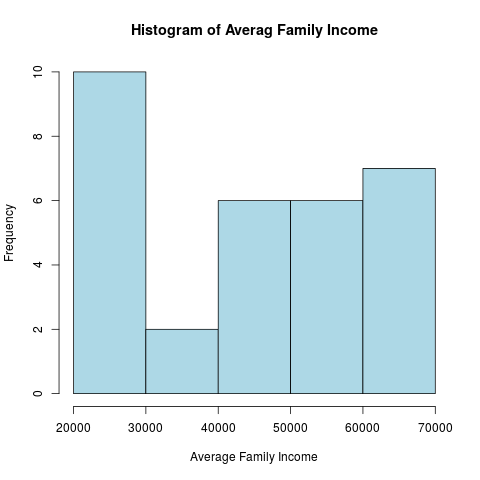
\includegraphics[width=0.5\textwidth]{histogram-income.png}
\caption{Average Family Income of Enrolled Students}

\paragraph{ Figure 2 shows enrollment rate vs average family income. Again we can see relatively two prominent peaks at 20-30K and 60-70K.  For people on the lower end of family income, studying art/design could be a relatively lucrative path given that arts, entertainment and design are big business in California. ( Hollywood down South and Berkeley/Santa Clara up North). For people on the higher end of family income, it's possible that they have been receiving high quality cultural/artsy education since young and has adequate family financial support to purse an artsy path.}

 \paragraph{ Figure 3 shows enrollment rate vs. gender, which simply indicates that for all 31 schools, female and male students populations are almost the same. }

\paragraph{Figure 4 shows enrollment ethnicity breakdown. The bar-plot indicates White and Hispanic make up half of the enrollment population. Since there aren't enough raw data available from College Scorecard (say ethnicity breakdown on average family income), it's difficult to extrapolate any other correlations (for example, could the 20-30K income peak corresponds to Hispanic enrollment?). Note that highest peak is "Other". This is because for simplicity, we combined all other race columns (except white, black, hispanic and asian) when producing the graphs. So "others" encompasses Indian-America, unknown, 2 or more race etc and thus the high percentage. }
  
  \paragraph{And finally, Figure 5 shows graduation rate ethnicity breakdown. Several things that need special attention. First, similar to Figure 4, the "Other" category includes multiple race options (it would be impractical to plot 12 bars into a single graph). Second, the total percentage of all bars don't add up to 1 due to nature of the clean data. For "Total" categories, it means the percentage of students that graduated within 4 years in total enrolled population. However, for "White", "Black", "Hispanic", "Asian" categories, it shows the percentage of students that graduated within their own racial category. (e.g about 45\% of white students graduated within 4 years in all white enrolled students). We comment that Hispanic and Asians have more than 50\% graduation rate while Black students suffer from low graduation rate. Again similar to Figure 4, due to deficiency of relevant data (e.g ethnicity vs average income), no other definitive conclusions can be drawn from the plot. }
  
  \paragraph{For a more quantitative data summary, we also include "eda-output-enroll" and "eda-output-grad" in the data file if readers are interested. }
 
  
 \section{Conclusion}
 \paragraph{In conclusion, through EDA analysis, we are able to provide a general overview of selected art institution in California regarding enrollment and graduation data. Through model building, we are able to show that there is a linear relationship between diversity variables and graduation rate in these art schools. Finally, we build an interactive shiny App for school administrators to visualize our analysis results }

\end{document}
